% !TeX root = ../main.tex
% Add the above to each chapter to make compiling the PDF easier in some editors.

\chapter{Introduction}\label{chapter:introduction}

The implemented low-level synchronization component in this Master's thesis is part of the KIA4SM project of the Chair of Operating Systems. The work aims to implement a method for dynamic update of task ready queues in L4 Fiasco.OC/Genode while providing a synchronized access to them.


\section{Overview of KIA4SM project}

KIA4SM (Cooperative Integration Architecture for Future Smart Mobility Solutions) is a research project at the Chair of Operating Systems \cite{kia4sm}. Traditionally, Cooperative Intelligent Transport Systems(C-ITS) have been built on heterogeneous systems. The KIA4SM project aims to provide an architecture of having a homogeneous software platform for heterogeneous hardware systems. The project focuses on developing systems for the interaction and coordination between partially or fully autonomously functioning computer-assisted vehicles. It also aims to improve the ad-hoc networking between vehicles.

The final vision of the project is illustrated in figure \ref{kia4sm}. The goals of the project are,

\begin{figure}[h]
  \centering
  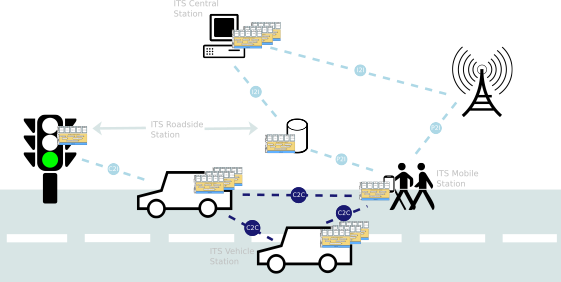
\includegraphics[scale = 1]{figures/kia4sm_vision.png}
  \caption{KIA4SM vision - homogeneous platform for heterogeneous be it  factors andT devices \cite{kia4sm}} \label{kia4sm}
\end{figure}

\begin{itemize}
%TODO rework
\item Providing a device independent platform. The different devices include vehicles, mobile devices of users and the supported devices for traffic and transport management.

\item Providing a mechanism for online dynamic reconfiguration, based on migration of software functionality, having a adaptive routing policy and flexible scheduling of tasks on the ECUs.
\end{itemize}

In order to achieve the goals of the project, a number of different methods have been applied such as application of the Organic Computing (OC) paradigm. The OC addresses the challenges of complex distributed systems by making them more life-like (organic) by endowing them with abilities such as self-organization, self-configuration, self-repair or adaptation \cite{branke2006organic}. In order to realize this, universally applicable Electronic Control Units (ECU) and a common run-time environment are used, which provide Hardware/Software Plug-and-Play properties.

\section{Motivation}

There are a number of micro controllers that are used for different calculations in a modern vehicle. The KIA4SM project aims to replace them with more powerful and standardized hardware, such as universally applicable ECUs. 

OC approach proposes a Observer-Controller architecture shown in figure \ref{architeture}, which is similar to the MAPE architecture (monitor, analyze, plan, execute). An observer collects the data from all the ECUs, computes and generates indicators. The controller then takes a decision based on the indicators and generates an action.

One such action of the controller is to decide the tasks that should be executed at a certain time in order to maintain the system in safe state. It is essential to be able to add threads and modify the execution order during operation time. Also, if an ECU is malfunctioning, thread migration is required. This involves swapping the threads from the malfunctioning one to the working ones. So, it is important to generate new ready-queues based on the information we receive from the other ECUs in the grid, and then exchange them with the actual ready-queue that the scheduler uses. There needs to be a method which allows to safely update the scheduler ready queue of the system. The work in this thesis concentrates on the scheduler ready queue update mechanism.

\begin{figure}[h][architecture]
  \centering
  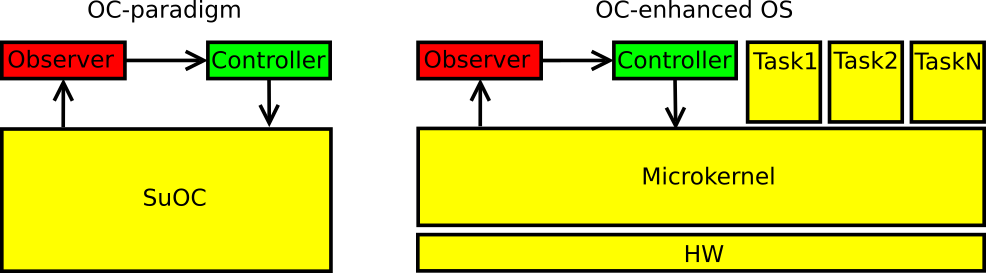
\includegraphics[scale = 0.5]{figures/microkernel_architecture.png}
  \caption{Organic Computing: Applying the Observer/Controller pattern to existing microkernel architecture \cite{kia4sm}}\label{architeture}
\end{figure}

\section{Thesis structure}
The thesis is structured in a inverted triangle model, the surrounding concepts are explained, before delving in to the specifics. 

The second chapter summarizes the related work on the state of the art algorithms for synchronization and different types of schedulers in use and at the end of the section an evaluation of the synchronization methods is provided in order to chose the best possible approach for the existing project.

The third chapter explains the Genode and L4 Fiasco.OC details in brief, in order for the user to have an overview of the system. 

The fourth chapter deals with the design details of synchronization module.

The fifth chapter explains the implementation of the design presented in the fourth chapter along with the code examples.  

The sixth chapter is dedicated to explain the testing method and the results obtained.
And the final chapter concludes the thesis with the limitations and future work to be done. 